% begin module improper-integral-type2-ex5
\begin{frame}
\begin{example} %[Example 5, p. 548]
Find $\displaystyle \alertNoH{4}{ \int_2^5 \alertNoH{3}{\frac{1}{\sqrt{x-2}} } \diff x} $.

\uncover<2->{Observe that $x = 2$ is a vertical asymptote for the integrand.}
\begin{columns}[c]
\column{.33\textwidth}
\psset{xunit=0.7cm, yunit=0.7cm}
\begin{pspicture}(-0.5, -0.5)(5.600000,3.3)
\psframe*[linecolor=white](-0.5,-0.5)(5.600000,3.3)
\tiny
\uncover<4->{\pscustom*[linecolor=\fcColorAreaUnderGraph]{
%Function formula: \frac{1}{(x-2)^{1/2}}
\psplot[linecolor=\fcColorGraph, plotpoints=1000]{2.100000}{5.000000}{1.0000000 -2.0000000 x add 0.5000000 exp div }
\psline(5.000000, 0)(2.00000, 0)(2,3.16227766)
}
}
\uncover<2->{\psline[linestyle=dashed](2, -0.49)(2, 3.19)}%
%Function formula: \frac{1}{(x-2)^{1/2}}
\uncover<3->{\psplot[linecolor=\fcColorGraph, plotpoints=1000]{ 2.1}{ 5}{1 -2 x add 0.5 exp div }}

\psaxes[arrows=<->](0,0)(-0.500000,-0.5)(5.5,3.2)
\fcLabels{5.5}{3.2}
\end{pspicture}


%\ 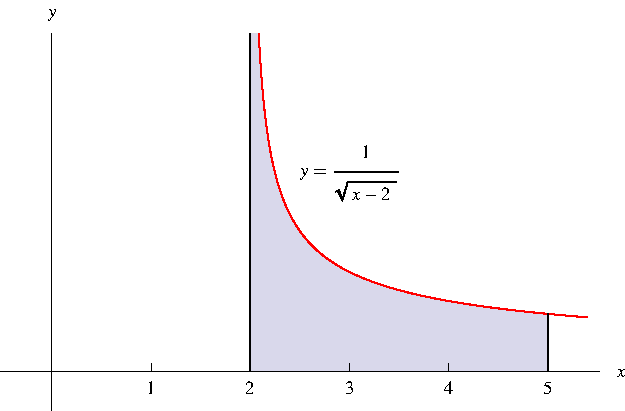
\includegraphics[height=4cm]{improper-integrals/pictures/08-08-ex5.pdf}%

\uncover<11->{Area = $2\sqrt{3}$}
\column{.67\textwidth}
\[
\begin{array}{@{}r@{}c@{}l}
\displaystyle \uncover<5->{%
\int_{\alertNoH{5}{2}}^5 \frac{1}{\sqrt{x-2}}\diff x%
}& \uncover<5->{ = } &\displaystyle %
\uncover<5->{%
\alertNoH{5}{\lim_{ t\rightarrow 2^+}} {\alertNoH{6,7}{\int}}_{\!\!\!\alertNoH{5}{t}}^5 \alertNoH{6,7}{\frac{1}{\sqrt{x-2}}\diff x}%
}\\%
& \uncover<6->{ = } &\displaystyle %
\uncover<6->{%
\lim\limits_{t\rightarrow 2^+}{\left[ \fcAnswer{7}{2\sqrt{x-2}}\right]}_{ \alertNoH{9}{ t}}^{\alertNoH{8}{ 5}}%
}\\%
& \uncover<8->{ = } &%
\uncover<8->{%
\lim\limits_{t\rightarrow 2^+} 2\left(\sqrt{\alertNoH{8}{5}-2} - \sqrt{\alertNoH{9}{t}- 2}\right)%
}\\%
& \uncover<10->{ = } &%
\uncover<10->{%
2\sqrt{3}%
}\\%
\end{array}
\]
\end{columns}
\end{example}
\end{frame}
% end module improper-integral-type2-ex5
